\chapter{\texorpdfstring{\MakeUppercase{Preston Royal Case Study}}{Preston Royal Case Study}}

Preston Royal Branch Library is a one-story building with
\SI{12400}{\feet\squared} of gross floor area. The library opened in 1954. The
facility consists of an open-space reading room and circulation, staff area,
and an auditorium.

The library is served by a single air handling unit. A BAS graphic of
the AHU is shown in \figref{} \ref{fig:PrestonRoyalAHUGraphic}. 

The AHU has 14 terminal units that serve the various areas of the
library and are shown in \figref{} \ref{fig:PrestonRoyalAHUGraphic} and
\ref{fig:PrestonRoyalTerminalUnitLayout}.

The terminal units are parallel fan powered boxes. A BAS graphic of one
of the terminal units is shown in \figref{}
\ref{fig:PrestonRoyalTerminalUnitGraphic}.

\begin{figure}
\centering
\includegraphics[width=\textwidth]{Images/PrestonRoyalAHUGraphic.PNG}
\caption{Preston Royal AHU BAS Graphic.}
\label{fig:PrestonRoyalAHUGraphic}
\end{figure}

\begin{figure}
\centering
\includegraphics[width=\textwidth]{Images/PrestonRoyalFPBLayoutGraphic.PNG}
\caption{Preston Royal terminal unit layout.}
\label{fig:PrestonRoyalTerminalUnitLayout}
\end{figure}

\begin{figure}
\centering
\includegraphics[width=\textwidth]{Images/PrestonRoyalTerminalUnitGraphic.PNG}
\caption{Preston Royal terminal unit graphic. }
\label{fig:PrestonRoyalTerminalUnitGraphic}
\end{figure}



\section{Preston Royal Zone Load Analysis}

The zone load profile for Preston Royal showed similarities to the NCTM
building. During operation, the estimated zone load fluctuated up and
down throughout the day. \figref{}
\ref{fig:2017-04-03-1250-ZoneLoadforFPB02-TikzData} shows an example of
how the zone load cycles up and down many times per hour. Again, the
hypothesized explanation for this is not that the actual heat gain in
the space is fluctuating, but that the HVAC controls are oscillating. 

\begin{figure}
\centering
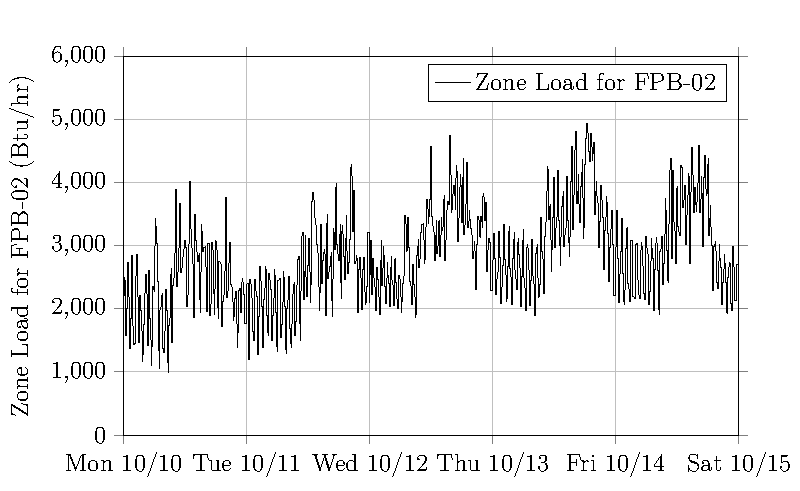
\includegraphics{Plots/2017-04-03-1250-ZoneLoadforFPB02-TikzData.pdf}
\caption{Zone load for FPB02 at Preston Royal Library.}
\label{fig:2017-04-03-1250-ZoneLoadforFPB02-TikzData}
\end{figure}


\figref{} \ref{fig:2017-06-05-0822-ZoneLoadforFPB02-TikzData} shows the
zone load for all the terminal units at Preston Royal Library for 3 days
from October 19\textsuperscript{th}, 2016 through October
21\textsuperscript{st}, 2016. Of interest to note is that within the
same space, one terminal unit can be experiencing a large cooling load
(FPB-11) while another terminal unit is calling for heating (FPB-08). 


\begin{figure}
\centering
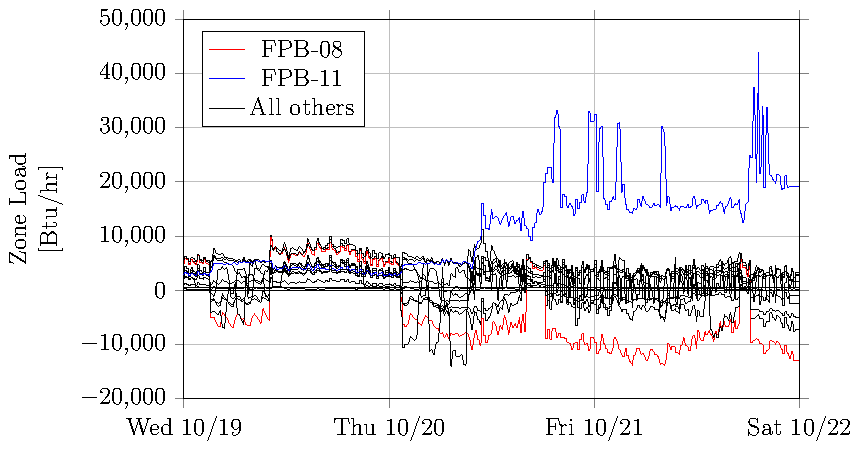
\includegraphics{Plots/2017-06-05-0822-ZoneLoadforFPB02-TikzData.pdf}
\caption{Zone load for all terminal units at Preston Royal Library.}
\label{fig:2017-06-05-0822-ZoneLoadforFPB02-TikzData}
\end{figure}


\newcommand{\prestonRoyalZoneLoadCaption}[1]{Zone load and prediction for #1.}
\begin{figure}
\centering
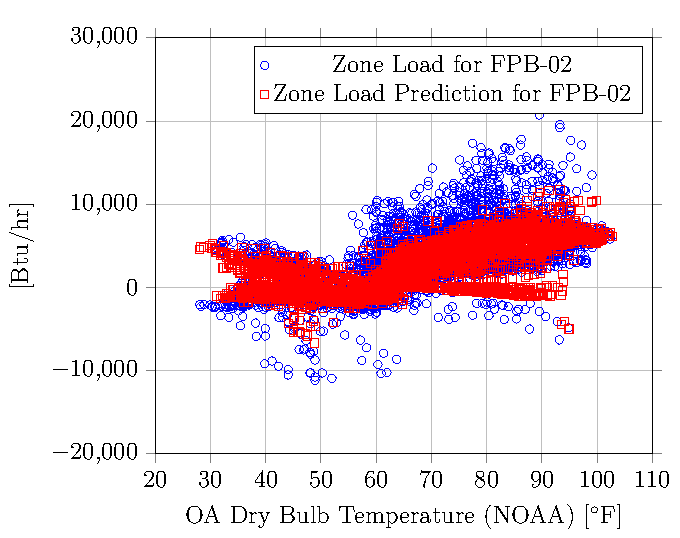
\includegraphics{Plots/37-PrestonRoyalFPB-02-ZoneLoad/2017-08-07-0816-BtuhrvsOADryBulbTemperatureNOAAF.pdf}
\caption{\prestonRoyalZoneLoadCaption{FPB-02}}
\label{fig:2017-08-07-0816-BtuhrvsOADryBulbTemperatureNOAAF}
\end{figure}

\begin{figure}
\centering
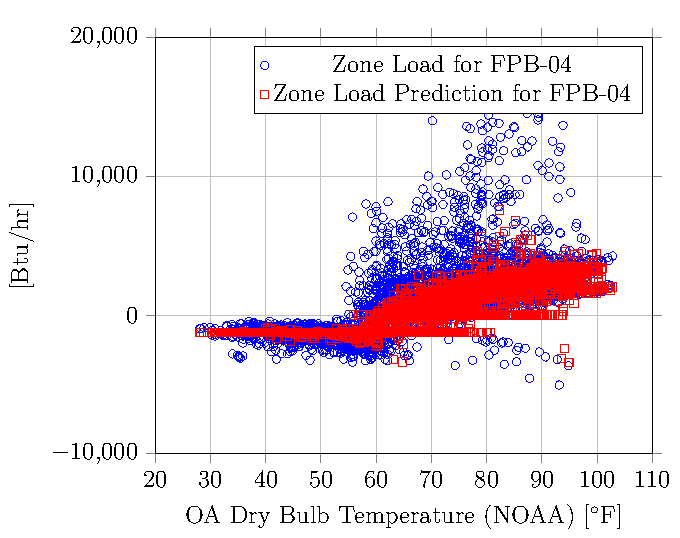
\includegraphics{Plots/38-PrestonRoyalFPB-04-ZoneLoad/2017-08-07-0917-BtuhrvsOADryBulbTemperatureNOAAF.pdf}
\caption{\prestonRoyalZoneLoadCaption{FPB-04}}
\label{fig:2017-08-07-0917-BtuhrvsOADryBulbTemperatureNOAAF}
\end{figure}

\begin{figure}
\centering
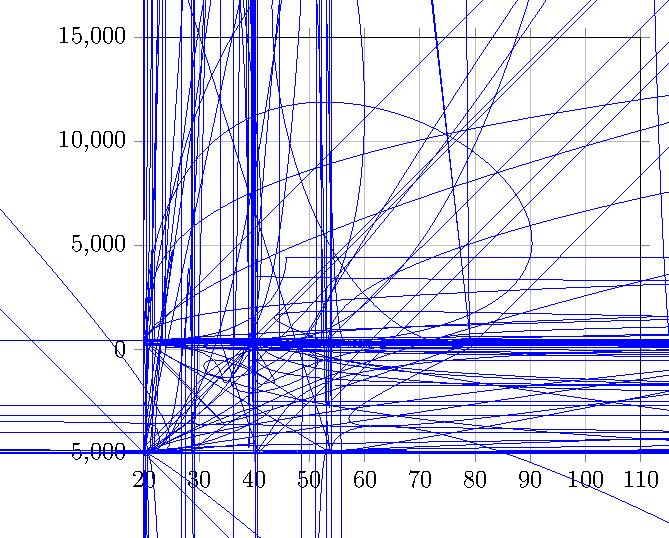
\includegraphics{Plots/39-PrestonRoyalFPB-06-ZoneLoad/2017-08-07-0922-BtuhrvsOADryBulbTemperatureNOAAF.pdf}
\caption{\prestonRoyalZoneLoadCaption{FPB-06}}
\label{fig:2017-08-07-0922-BtuhrvsOADryBulbTemperatureNOAAF}
\end{figure}

\begin{figure}
\centering
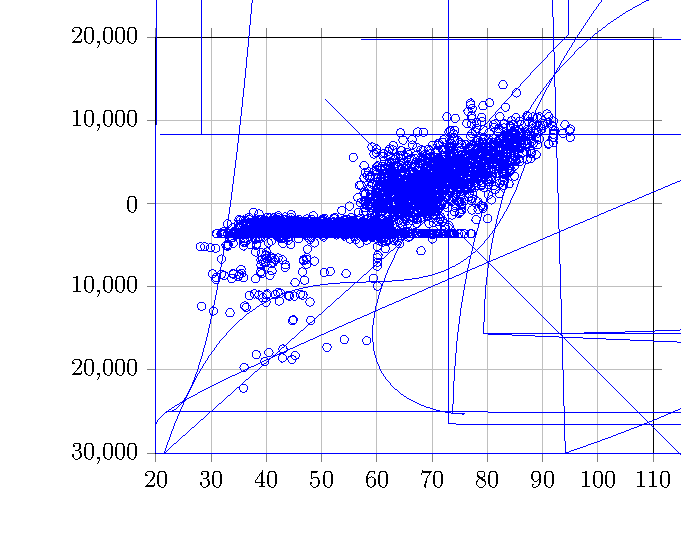
\includegraphics{Plots/40-PrestonRoaylFPB-07-ZoneLoad/2017-08-07-0927-BtuhrvsOADryBulbTemperatureNOAAF.pdf}
\caption{\prestonRoyalZoneLoadCaption{FPB-07}}
\label{fig:2017-08-07-0927-BtuhrvsOADryBulbTemperatureNOAAF}
\end{figure}

\begin{figure}
\centering
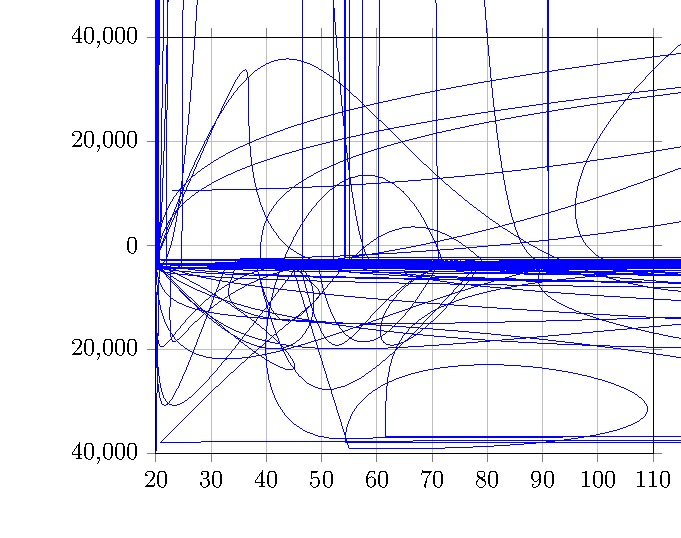
\includegraphics{Plots/41-PrestonRoyalFPB-08-ZoneLoad/2017-08-07-0927-BtuhrvsOADryBulbTemperatureNOAAF.pdf}
\caption{\prestonRoyalZoneLoadCaption{FPB-08}}
\label{fig:2017-08-07-0927-BtuhrvsOADryBulbTemperatureNOAAFFPB-08}
\end{figure}

\begin{figure}
\centering
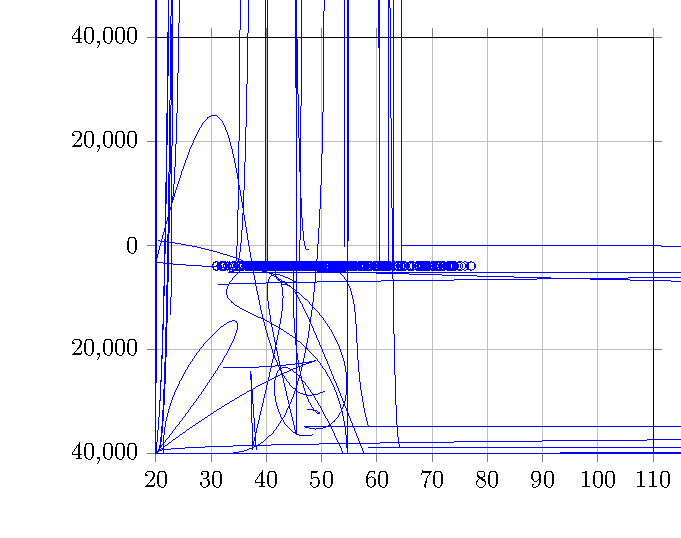
\includegraphics{Plots/42-PrestonRoyalFPB-09-ZoneLoad/2017-08-07-0928-BtuhrvsOADryBulbTemperatureNOAAF.pdf}
\caption{\prestonRoyalZoneLoadCaption{FPB-09}}
\label{fig:2017-08-07-0928-BtuhrvsOADryBulbTemperatureNOAAF}
\end{figure}

\begin{figure}
\centering
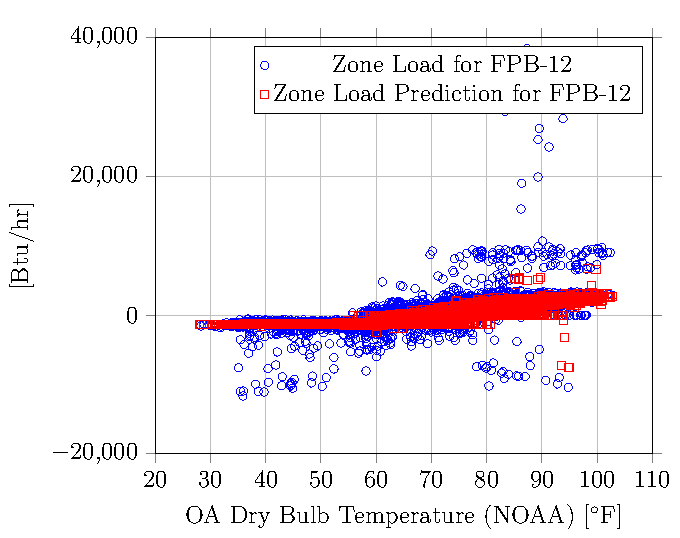
\includegraphics{Plots/43-PrestonRoyalFPB-12-ZoneLoad/2017-08-07-0928-BtuhrvsOADryBulbTemperatureNOAAF.pdf}
\caption{\prestonRoyalZoneLoadCaption{FPB-12}}
\label{fig:2017-08-07-0928-BtuhrvsOADryBulbTemperatureNOAAF12}
\end{figure}

\section{Estimated Savings}

Only 7 of the 14 air handling units had usable data. The estimated
savings from this pseudo-synthetic data set was examined. A portion of
the library was able to be optimized, utilizing several
assumptions were made in order to make the analysis possible. 

\begin{itemize}
    \item There was no mixed air temperature sensor available, so the
        mixed air temperature was assumed to be between the outdoor air
        temperature and the return air temperature with the following
        relationship
\begin{equation}
\mat{} = 0.3 \oat{} + 0.7 \rat{}
\end{equation}
\item The mixed air humidity ratio was also not known. It was assumed to
    have a similar relationship as the mixed air temperature, however,
    during times of low humidity, the mixed air humidity ratio will just
    be the outdoor air humidity ratio
\begin{equation}
    \omega_{ma} = \text{MIN}\left(\omega_{oa}, 0.3 \omega_{oa} + 0.7
    \omega_{sa}\left(\sat{}\right) \right)
\end{equation}
\item The minimum flow rate percentage for the terminal units was
    assumed to be 30\%. 
\end{itemize}

Data existed from December 1\textsuperscript{st}, 2015 to October
22\textsuperscript{nd}, 2016. Timestamps when the air handling unit was
off were ignored. 

Times when the actually supply air temperature was out of a reasonable
range was also ignored. 

Over the course of the approximately 323 day period, the potential
percent dollar savings was 15\%. In general, the savings were due to
raising the supply air temperature, which while increasing the total fan
energy, decreased the required cooling and reheat energy. 

The cost of sensible cooling was the largest component, over 50\% for
both the actual and optimal operations. 

\begin{table}
\centering
\caption{Estimated savings from the partial data set originating from Preston Royal library.}
\label{tab:prestonRoyalSavings}

\begin{tabular}{lllS}
\toprule
    Component               & { Estimated Actual (\$) } & { Optimal (\$) }     & { Savings (\$) } \\ \midrule
    Fan Energy              & \num{431.28} (11\%)       & \num{563.30} (17\%)  & -132.02          \\
    Sensible Cooling Energy & \num{2222.51} (55\%)      & \num{1986.98} (59\%) & 235.53           \\
    Latent Cooling Energy   & \num{642.57} (16\%)       & \num{461.60} (14\%)  & 180.97           \\
    Reheat Energy           & \num{717.27} (18\%)       & \num{376.87}  (11\%) & 340.4            \\ \midrule
    Total                   & \num{4013.64}             & \num{3388.75}        & 623.457          \\ \bottomrule
\end{tabular}

\end{table}



